\documentclass[a4paper]{article}

\usepackage[english]{babel}
\usepackage[utf8x]{inputenc}
\usepackage{amsmath}
\usepackage{graphicx}
\usepackage{placeins}
\usepackage{float}



\usepackage[colorinlistoftodos]{todonotes}
\usepackage{titling}
\setlength{\droptitle}{-4.5cm}
\usepackage{amssymb}
\usepackage{algorithm,algpseudocode}
\usepackage{subfig}
\usepackage{bm,nicefrac}
\usepackage{comment}


\newtheorem{mydef}{Definition}
\newtheorem{myremark}{Remark}



\usepackage{hyperref}
\hypersetup{
    colorlinks=true,
    linkcolor=blue,
    filecolor=magenta,      
    urlcolor=cyan,
}






\title{Parallelizing the Exact test}
\author{Markus Ekvall, Micheal Höhle, and Lukas Käll}

\addtolength{\textwidth}{1.8cm}

\begin{document}
\tableofcontents
\maketitle

\section{Abstract}
The exact test is common practice within life sciences; however, it is slow to compute since the runtime grows combinatorially with a naive implementation. Nevertheless, continued development in the 1980s  led to a dynamic programming algorithm that computes the exact test in polynomial time. Albeit this significant run time reduction, the exact test has not yet become one of the predominant statistical tests for larger set-sizes. However, some further refinement could make the algorithm even faster–since it could become parallelizable–henceforth, making the exact test more attractive. Parallelization is possible by some nontrivial rearrangement of the structure of the algorithm. Making the computation parallel on a GPU gains additional orders of magnitude of speedup of this algorithm. Hence, the runtime of the exact test would essentially become a non-issue.

\section{Introduction}
The exact permutation test is a standard tool within life sciences and is especially valuable when the sample size is too small to use the asymptotical test. However, the exact test is unattractive computationally \cite{segal2018fast}. Nonetheless, this computational unattractiveness has been partially solved by a theorem by \cite{pagano_trichtler1983} and inspired a dynamic programming algorithm that has been made explicit by \cite{zimmermann1985}. This algorithm is effective compared with any naive approach; nevertheless, the popularity of the exact test for larger set sizes has not increased since this improvement. However, further refinement of the algorithm–it can be made parallelizable–could make it a more widely popular statistical tool.

Here's the sections of this paper: Firstly, the main objective–how to compute $p$-values with an exact test–is described in section \ref{sec:PvalueComputation}, a detailed explanation of the algorithm is presented in section \ref{sec:calcBottleneck}, a further description how this algorithm can be parallelizable is presented in section \ref{sec:paraAlgo}, and, finally, the result section \ref{sec:result}, comparing the empirical runtimes between the non-parallelized version and parallelized version.

\section{$P$-value computation}
\label{sec:PvalueComputation}
\subsection{Setup}
Let $\bm{x}=(x_1,\ldots, x_m)$ and $\bm{y}=(y_1,\ldots,y_n)$ be two samples consisting of integer values, i.e. $x_i \in \mathbb{N}_0$ for $1\leq i \leq m$ and $y_j \in \mathbb{N}_0$ for $1\leq j\leq n$. Then the observed sum of sample $\bm{x}$ is $s_{\text{obs}} = \sum_{i=1}^m x_i$ and one would like to know how extreme $s_{\text{obs}}$ is under the null hypothesis (i.e., that the mean does not differ between the two distributions) against the alternative hypothesis (i.e., that the mean in the second group is larger than in the first group); this is equivalent to investigate the likelihood to observe $s_{obs}$ or a more extreme value in the direction of the alternative hypothesis – known as the $p$-value. More formally, the $p$-value is: $P(s_{\text{obs}} \leq S | \bm{x}, \bm{y})$, where $P(S)$ is the probability mass function and $S$ is a random variable denoting the value of the sum in the first sample under the permutation distribution. The computationally expensive part is to obtain $P(S)$ which is estimated by concatenating $\bm{x}$ and $\bm{y}$ to $\bm{z}=(x_{1},\ldots,x_{m},y_{1},\ldots,y_{n})=(z_1, z_2, \ldots, z_{n+m})$, and draw all possible combinations of length $m$ from $\bm{z}$ and count the number of occurrences of all possible sums; when the numbers of occurrences of all possible sums are available, the distribution is accessible. The concept of combination will be instrumental, ergo, worth explicitly define for the general case.

\begin{mydef}[$j$-combination] The $j$-combination of a set $\bm{z}$ is a subset with $j$ distinct elements where order does not matter.\end{mydef}

The maximal sum obtained from a $m$-combinations of $\bm{z}$ is $\mathcal{S}$ (i.e., a combination containing the $m$ largest values in $\bm{z}$); hence, the possible states of the integer sum of any $m$-combinations are $\Omega=\{0,1,\ldots,\mathcal{S}\}$ (recall that $z_{i}\in \mathbb{N}_0$ ), which denotes the support of the sum. Assume a random variable $\bm{z}^{*}=(z^{*}_1,\ldots,z^{*}_m)$, that is a randomly sampled $m$-combination from $\bm{z}$ and its corresponding sum is $S=\sum_{i=1}^m z^{*}_i$, where $S\in \Omega$. Then $P(S)$:

\begin{align}
\label{eq:pOfS}
P(S = s) &= \frac{\text{\# $m$-combinations of $\bm{z}$ s.t. sum is equal to $s$}}{\text{\# $m$-combinations of $\bm{z}$}}, 
\end{align}
where $0\leq s \leq \mathcal{S}$. From basic combinatorics the denominator of the above equation \ref{eq:pOfS} is equal to:

\begin{align*}
{m+n \choose m} = \frac{(m+n)!}{n!m!}
\end{align*}

The calculation of the numerator is the intricate part (e.g., a naive algorithm that would exhaustively check the sum for each possible $m$-combinations and compare it to $s$, for all $s$, would take $\mathcal{O}(\mathcal{S} \cdot {m+n \choose m})$, i.e., a combinatorial explosion) and how to set-up an efficient algorithm with polynomial time complexity is further discussed in section \ref{sec:calcBottleneck}. However, for the sake of discussion, here is the definition of the general case of the numerator.
\begin{mydef}[$N(s,j)$]
\label{def:numerator}
$N(s,j)$=\# $j$-combinations of a set $\bm{z}$ s.t. their elements sum is equal to $s$.
\end{mydef}

By definition \ref{def:numerator}, the specific numerator in equation \ref{eq:pOfS} is then $N(s,m)$, and when attained, the sought $p$-value can be calculated as:

\begin{align}
P(s_{\text{obs}} \leq S | \bm{x}, \bm{y}) &= \sum _{s=s_{obs}}^{\mathcal{S}}\frac{N(s,m)}{{m+n \choose m}}=\sum _{s=s_{obs}}^{\mathcal{S}}P(s)
\end{align}

As mentioned above, there is no trivial method to obtain $N(s,m)$. However, it is possible to develop a  dynamic programming algorithm to obtain $N(s,m)$ \cite{pagano_trichtler1983, zimmermann1985}, which is described thoroughly in the next section.

\section{Dynamic programming: Calculate the Number of $m$-combinations s.t. their sums equal $s$. i.e., $N(s,m)$}
\label{sec:calcBottleneck}

As an introduction, the dynamic programming algorithm was first implemented and proved by \cite{zimmermann1985, pagano_trichtler1983}. Therefore, the correctness of the algorithm is not under scrutiny in this section. However, a great deal of effort is exerted to explain the algorithm, which is necessary to describe its parallelizability in section \ref{sec:paraAlgo}.

To solve for $N(s,m)$ efficiently, one would like to find a relation between $N(s,m)$ and a simpler case of itself–i.e., find a recurrence relation. There is no apparent such relation for the general case $N(s,j)$, see definition \ref{def:numerator}. However, by considering fewer elements of $\bm{z}$ it is possible to start from a simple case, then successively build up to more complex cases.

\begin{mydef}
\label{def:specificNumerator}
\begin{align*}
N(s,i,j)&=\textit{\# j-combinations from $z[1,\ldots,i]$ s.t. the sum is equal to $s$}\\
        &=\textit{\# j-combinations from $z[1,\ldots,i]$ s.t. $\sum _{l=1}^{j}z_{l}=s$}
\end{align*}
\end{mydef}
\begin{myremark}
\label{rm:finalN}
For a set $|\bm{z}|=k$, then $N(s,i=k,j)=N(s,j)$, since $\bm{z}[1,\ldots,k]=\bm{z}$, hence, definition \ref{def:numerator} and definition \ref{def:specificNumerator} are compatible.
\end{myremark}

It follows directly from definition \ref{def:specificNumerator}: If $i<j$, i.e., when considering fewer elements in $\bm{z}$ than elements required to form a $j$-combinations, then it can trivially not exist any such combination. Moreover, a second observation is that $N(s,i,j)$ has to be zero when either $i=0$ (i.e., checking the empty set of $\bm{z}$.) or $s < 0$, or when $\mathcal{S} < s$ (i.e., when $s$ is outside the boundary of possible sums.). These conditions will form the boundary conditions:

\begin{align}
\label{eq:Subrecursion1}
N(s,i,j) &=0, & \text{if $i < j$, $i=0$, $s < 0$, or $\mathcal{S} < s$.}
\end{align}

The expression of $N(s,i,j)$ in definition \ref{def:specificNumerator} is not yet especially helpful, but since it is possible to consider fewer elements of $\bm{z}$, it is possible to re-factoring the expression:

\begin{align*}
N(s,i,j) &= \textit{\# $j$-combinations from $z[1,\ldots,i]$ s.t. $\sum _{l=1}^{j}z_{l}=s$} \\
        &= \textit{\# $j$-combinations from $z[1,\ldots,(i-1)]$ s.t. $\sum _{l=1}^{j}z_{l}=s$} \\
        &+ \textit{\# $j$-combinations from $z[1,\ldots,i]$ s.t. $\sum _{l=1}^{j}z_{l}=s$ and contains $z_{i}$.} \\
        &= N(s,i-1,j)+ \phi (s,i,j) \\
\end{align*}

Now $N(s,i,j)$ is written in it's first primitive recursive form, i.e.,
\begin{align}
\label{eq:recursion1}
N(s,i,j) = N(s,i-1,j)+ \phi (s,i,j) 
\end{align}

With a placeholder-function that yet has to be decided explicitly, i.e.,

\begin{align}
\label{eq:cond2}
\phi (s,i,j) &= \textit{\# $j$-combinations from $z[1,\ldots,i]$ s.t. $\sum _{l=1}^{j}z_{l}=s$ and contains $z_{i}$.}
\end{align}

Now, something more practical start to reveal itself; only $\phi (s,i,j)$ left to determine. This function $\phi (s,i,j)$ will differ for $j$-combinations with one element (i.e., $j=1$.), and those with more elements (i.e., $j>1$.). Here is a formal description of the first case (i.e., $j=1$.): Since there is only one element in a $1$-combination, then either $z_{i}=s$ or it is not. Thus,

\begin{align}
\label{eq:cond3}
\phi (s,i,j=1) &=\begin{cases}
    1, & \text{if $j=1$ and $z_{i}=s$}.\\
    0, & \text{if $j=1$ and $z_{i}\neq s$}.
  \end{cases}
\end{align}

Combine the recursive form \ref{eq:recursion1} with condition \ref{eq:cond3} to obtain the sub-recursion below:

\begin{align}
\label{eq:Subrecursion2}
N(s,i,j) &=\begin{cases}
    N(s,i-1,j)+1, & \text{if $j=1$ and $z_{i}=s$}.\\
    N(s,i-1,j), & \text{if $j=1$ and $z_{i}\neq s$}.
  \end{cases}
\end{align}

So far, the sub-recursion \ref{eq:Subrecursion1} and \ref{eq:Subrecursion2} form the base-cases, now it is time to determine the generic recursion containing $\phi (s,i,j>1)$ (i.e., for combinations with more than one element). This one is trickier to explain than the other ones, so here's an example for some intuition: Say that the only $2$-combinations summing up to $5$ are $\{2,3\}$ and $\{0,5\}$ in $z[1,\ldots,4]$, and hence $N(5,4,2)=2$ (see definition \ref{def:specificNumerator}). Furthermore, when extending $z[1,\ldots,5]$ where $z_{5}=5$, by the assertion in the previous line, the only $3$-combinations summing up to $10$ that contains $z_{5}$ is $\{2,3\} \cup {z_{5}}$ and $\{0,5\} \cup {z_{5}}$, and therefore $\phi (10,5,3)=2$ (see definition \ref{eq:cond2}). The crucial observation is that there is an equivalence $\phi (10,5,3)=N(5,4,2)$ .

For the general case, say that $N(s - z_{i},i-1,j-1)$ is known. Thus, by adding $z_{i}$ to all those $(j-1)$-combinations summing up to $(s - z_{i})$ counted by $N(s - z_{i},i-1,j-1)$, the number of $j$-combinations summing up to $s$ that contains $z_{i}$ which $\phi (s,i,j)$ ought to count is revealed–namely $N(s - z_{i},i-1,j-1)=\phi (s,i,j)$, given $z_{i} \leq s$, since there exist no $s<0$.
\begin{align}
\label{eq:cond4}
\phi (s,i,j) &=\begin{cases}
    N(s - z_{i},i-1,j-1), & \text{if $j>1$ and $z_{i} \leq s$}.\\
    0, & \text{if $j>1$ and $s < z_{i}$}.\\
  \end{cases}
\end{align}

Again, combine recursion \ref{eq:recursion1} with condition \ref{eq:cond4} to obtain the generic sub-recursion below.

\begin{align}
\label{eq:Subrecursion3}
N(s,i,j) &=\begin{cases}
    \text{$N(s,i-1,j)$ + $N(s-z_{j},i-1,j-1)$}, & \text{if $j>1$ and $z_{i} \leq s$}.\\
    \text{$N(s,i-1,j)$}, & \text{if $j>1$ and $s < z_{i}$}.\\
  \end{cases}
\end{align}

By combining the base-case sub-recursions \ref{eq:Subrecursion1} and \ref{eq:Subrecursion2} with the generic sub-recursion \ref{eq:Subrecursion3}, the final recursion is:

\begin{align}
\label{eq:finalRecursion}
\text{$N(s,i,j)$}   =\begin{cases}
    0, & \text{if $i < j$, $i=0$, and $s < 0$.} \\
    \text{$N(s,i-1,j)$}+1, & \text{if $j=1$ and $z_{i}=s$}.\\
    \text{$N(s,i-1,j)$}, & \text{if $j=1$ and $z_{i}\neq s$}. \\
    \text{$N(s,i-1,j)$ + $N(s-z_{j},i-1,j-1)$}, & \text{if $j>1$ and $z_{i} \leq s$}. \\
    \text{$N(s,i-1,j)$}, & \text{if $j>1$ and $s < z_{i}$}. \\
  \end{cases}
\end{align}

Below is a top-down algorithm of the recursion \label{eq:finalRecursion}.

\FloatBarrier
\begin{algorithm}
\caption{\# $j$-combinations s.t. their elements sum is equal to $s$.}
\label{alg:combination}
\begin{algorithmic}[1]
\State $m$: Scalar equal to the number of samples in $x$.
\State $n$: Scalar equal to the number of samples $y$.
\State $\mathcal{S}$: Scale equal to the sum of the $m$ largest values in $z$.
\State $z$: Concatenated vector of $x$ and $y$ with length $m+n$.
    \Procedure{NumberOfCombinations}{$m$, $n$, $\mathcal{S}$, $z$}
    \State Allocate array $N_{i-1}[0...\mathcal{S},0...m]$ with zeros 
    \State Allocate array $N_{i}[0...\mathcal{S},0...m]$ with zeros
    \For{$i=1$ to $(m + n) +1$}
        \For{$j=1$ to $m+1$}
            \For{$s=1$ to $\mathcal{S} +1$}
                \If{$i < j$} \Comment{Sub-recursion \ref{eq:Subrecursion1}} \State $N_{i}[s,j-1]=0$ 
                \ElsIf{$j==1$ and $z[i-1] == s$} \Comment{Sub-recursion \ref{eq:Subrecursion2} } \State $N_{i}[s,j-1]=N_{i-1}[s,j-1] + 1$
                \ElsIf{$j==1$ and $z[i-1] \neq s$} \State $N_{i}[s,j-1]=N_{i-1}[s,j-1]$ 
                \ElsIf{$j>1$ and $z[i-1] \leq s$} \Comment{Sub-recursion \ref{eq:Subrecursion3} } \State $N_{i}[s,j-1]=N_{i-1}[s-z[i-1],j-2] + N_{i-1}[s,j-1]$ 
                \ElsIf{$j>1$ and $z[i-1] > s$} \State $N_{i}[s,j-1]=N_{i-1}[s,j-1]$
                \EndIf
            \EndFor
        \EndFor
        \State $N_{i-1} = N_{i}$; \Comment{Update $N_{i-1}$ for next iteration.}
    \EndFor
        \State \Return $N_{i}[0...\mathcal{S},m]$ \Comment{By remark \ref{rm:finalN}: N_{m+n}[s,m]=N(s,m)$}
        
    \EndProcedure
\end{algorithmic}
\end{algorithm}
\FloatBarrier
The algorithm needs some explanation. Instead of using one extensive array $N[0\ldots \mathcal{S},$\ $0\ldots(m+n),0\ldots m]$, two smaller arrays, $N_{i-1}[0...\mathcal{S},0...m]$ and $N_{i}[0...\mathcal{S},0...m]$, are swapped and rewritten in each iteration of $i$ in an oscillatory fashion – to save memory. Notice that $N_{i}$ is not required to reset after line $24$ (this is especially nice on a GPU since there is no easy way to reset the entries.); this is possible since nothing is dependent on $N_{i}$ in the next iteration $i+1$, and any of the conditions between line $11$ and $19$ will entirely rewrite $N_{i}$ so it will be correct at $i+2$, where it will be used. 
The reason that the latter approach saves memory is due to the former array requires $\mathcal{O}(\mathcal{S} \cdot (m+n) \cdot m)$, whereas the latter two arrays require $\mathcal{O}(\mathcal{S} \cdot m + \mathcal{S} \cdot m) = \mathcal{O}( 2 \cdot \mathcal{S} \cdot m)=\mathcal{O}(\mathcal{S} \cdot m)$. Moreover, this improvement in memory usage is a quintessential difference for the parallelized algorithm (the memory storage of the GPU can easily be a bottleneck). 
A second point, notice the structure of the for-loops; they could easily have been arranged in whatever way and still obtain correct computations. However, the dimensions of the two arrays have to be adjusted appropriately related to the outer-most loop. Nevertheless, this specific order has a purpose–it is parallelizable–which will be described in the next section.
One final note on algorithm \ref{alg:combination}, by plain observation on the nested loops, it easy to see that the runtime is $\mathcal{O}(m\cdot (m+n)\cdot \mathcal{S})$.
Here's a demonstration of one iteration of $i$, to make the mechanics of algorithm \ref{alg:combination} even clearer.
\begin{figure}[H]
\centering
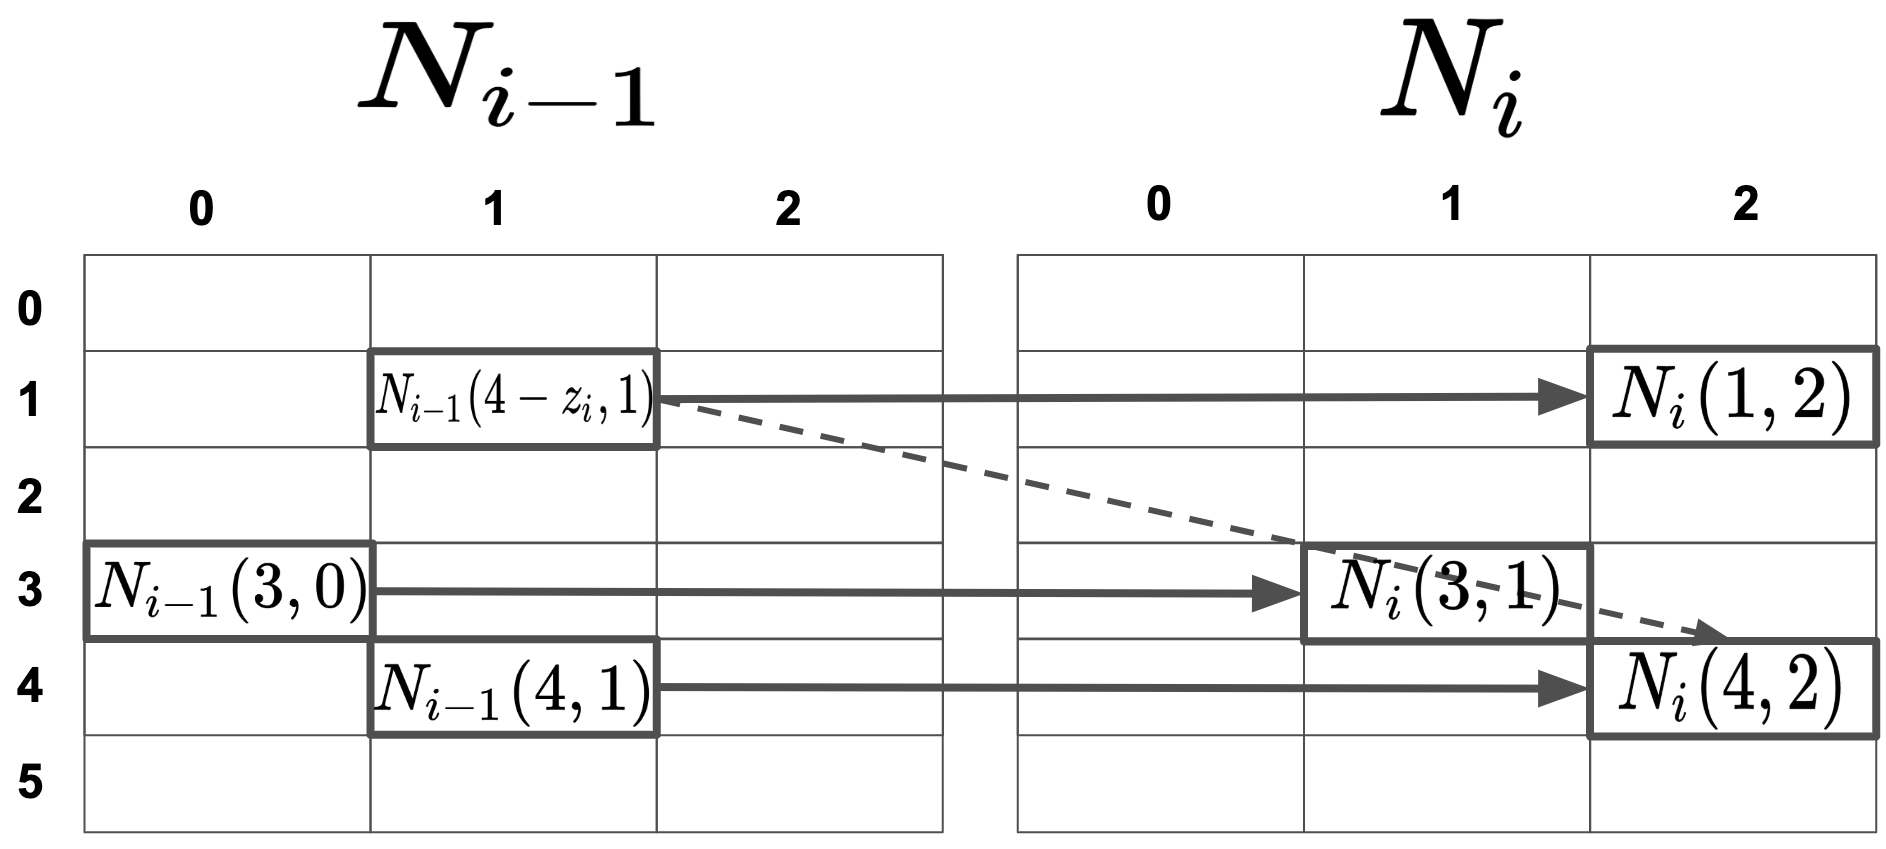
\includegraphics[height=0.45\textwidth]{exampleparallelized.png}
\caption{Demonstration the computations of three entries of $N_{i}$.}\label{normal_calibration.png}
\end{figure}
The figure demonstrates three different calculations and all applies different conditions in recursion \ref{eq:finalRecursion}. Firstly, in the right array $N_{i}$, see entry $N_{i}(4,2)$, the arrows from $N_{i-1}$ indicates that it is dependent on entries $N_{i-1}(4,1)$ and $N_{i-1}(1=4-z_{i},1)$ from array $N_{i-1}$. The reason is that the entry $N_{i}(4,2)$ considers more than one element of $z$ (i.e., $j>1$), and the sum $s=4$ is more than $z_{i}=3$ (i.e.,. $s>z_{i}$). Hence, by condition \ref{eq:Subrecursion3}, by adding $N_{i-1}(4,1)$ and $N_{i-1}(1=4-z_{i},1)$ one obtains $N_{i}(4,2)$ (i.e., $N_{i}(4,2)=N_{i-1}(4,1) +N_{i-1}(1=4-z_{i},1)$). 
In the second example, see entry  in $N_{i}(3,1)$, it is only dependent on $N_{i-1}(3,0)$, and this is because it is only concerned with one element in $z$ (i.e., $j=1$). Furthermore, since $z_{i}=s=3$ one should apply condition $\ref{eq:Subrecursion2}$. Hence, one obtains $N_{i}(3,1)$ by adding $N_{i-1}(3,0)$ with one (i.e., $N_{i}(3,1)=N_{i-1}(3,0)+1$). 
Finally, see entry $N_{i}(1,2)$ in $N_{i}$, it is solely dependent on $N_{i-1}(1,1)$ because it considers more than one element in $z$ $(i.e., j>1)$, and the sum $s=2$ is less than $z_{i}=3$ (i.e., $s<z$). Thus, by condition \ref{eq:Subrecursion3},  $N_{i}(1,2)$ is obtained by taking $N_{i-1}(1,1)$ (i.e., $N_{i}(1,2)=N_{i-1}(1,1)).$
\section{Parallelization of algorithm}
\label{sec:paraAlgo}
The algorithm in section \ref{alg:combination} perfectly parallelizable, but not trivially so. To achieve parallelizing, one needs to be very explicit about the choice of the nesting of the loops. The rest of this section will demonstrate the reason why.
The first thing to check is if the algorithm is parallelizable over all three dimensions, i.e., $s, i$, and $j$, which would be preferable. However, there exist several counterexamples that no such parallelization exist, but one example is sufficient, described in section \ref{sec:3Dpara}. Fortunately, the algorithm is parallelizable over the two variable $s$ and $j$, described in section \ref{sec:2Dpara}.
\subsection{Parallelization over three dimensions: $s, i$, and $j$.}
\label{sec:3Dpara}
Observe sub-recursion \ref{eq:Subrecursion2}. Keep in mind, the whole array $N[0\ldots \mathcal{S},$\ $0\ldots(m+n),0\ldots m]=0$ at the beginning, see algorithm \ref{alg:combination}.  At some point, the algorithm has to go through all the cases for $j=1$, and at least once $z_{i}=s$ (otherwise $\bm{z}$ would be an empty array) for some $i$. Hence, $N(s,i,1) = N(s,i-1,1)+1$. Meanwhile, the computation of $N(s,i+1,1)$ is done on another process, not aware of the update of $N(s,i,1)$. Therefore interpreting $N(s,i,1)=0$, but in fact, $N(s,i,1)>1$. Consequently, $N(s,i+1,1)$ that is dependent on $N(s,i,1)$ will be wrong. Since there is no assurance that these cases compute correctly, the conclusion is that the algorithm \ref{alg:combination} is not parallelizable over $i,j$, and $k$.
It is possible to build up the same argument for recursion \ref{eq:Subrecursion3}, and it all boils down to $N(s,i,j)$ is going to depend on computations made in parallel, and hence not available at the time for computation of $N(s,i,j)$.
\subsection{Parallelization over two dimensions: $s$ and $j$}
\label{sec:2Dpara}
The meaning of parallelizing over two dimensions, is, in this case, to fix one of the variables and check whether the two other variables are parallelizable given the third fixed variable. In practice, the fixed variable is the outer most for-loop, and for each iteration of this variable, then within this loop, everything is calculated in parallel over the two other variables.
Out of the three variables, it is only necessary to find one such variable to fix, and instead of exhaustively check all possibilities, one can check recursion \ref{eq:finalRecursion} to see which variable is parallelizable. By comparing the left side to the right side, the only variable that is not dependent on contemporary action of itself is variable $i$ i.e., $N(s,i,j)=f(s,s-z_{j},i-1,j,j-1)$, and, furthermore, the other two variables is not possible to fix. Below is a verification that $N(s,i,j)$ is parallelizable given that $i$ is fixed.
\newline
\begin{comment}
\subsubsection{Initiation: $i=0$}
\label{subsubsec:v1}
Recursion \ref{eq:Subrecursion1} (i.e., when $i=0$) is trivially parallelizable since it is not dependent on any previous calculations.
\end{comment}
\subsubsection{Initiation: $i=1$}
\label{subsubsec:v2}
In line $6-7$ in algorithm \ref{alg:combination}, both arrays $N_{1}[0...\mathcal{S},0...m]$ and $N_{0}[0...\mathcal{S},0...m]$ are initialized with zeros. When $i=1$, the only possible conditions are those between the lines $11-16$, i.e., sub-recursion \ref{eq:Subrecursion1} and \ref{eq:Subrecursion2}. Sub-recursion \ref{eq:Subrecursion1} is trivially parallelizable since it is not dependent on any previous calculations. The only pre-computed values required for sub-recursion \ref{eq:Subrecursion2} is from $N_{0}[0...\mathcal{S},0...m]$, which is available. Hence, sub-recursion \ref{eq:Subrecursion2} is parallelizable. Since all possible condition at $i=1$ is parallelizable, one can conclude that the algorithm is completely parallelizable at $i=1$.
\subsubsection{Maintenance: $2\leq i \leq (m+n)+1$}
\label{subsubsec:maintenance}
Between leaving iteration $i$ (e.g., $i=1$) and before incrementing $i\leftarrow i+1$ (e.g., updating $i$ to $i=2$), the algorithm updates $N_{i-1}$=$N_{i}$ at line $24$. When entering iteration $(i+1)$ all conditions (i.e., those between line $11-20$) are possible, i.e., sub-recursion \ref{eq:Subrecursion1}, \ref{eq:Subrecursion2}, and \ref{eq:Subrecursion3}. However, one can reuse the same arguments from the previous section \ref{subsubsec:v2} for both conditions \ref{eq:Subrecursion1} and \ref{eq:Subrecursion2}, since $N_{i-1}$ (e.g., $N_{1}[0...\mathcal{S},0...m]$) are available. For the last condition, sub-recursion \ref{eq:Subrecursion3} is only dependent on $z[1,\ldots,m+n]$ and $N_{i-1}$. As mentioned, $N_{i-1}$ is available, and $z$ is available since it is an invariant. Thus, sub-recursion \ref{eq:Subrecursion3} is parallelizable. Since all possible conditions at iteration $(i+1)$ are parallelizable, one can assert that the algorithm is fully parallelizable at iteration $(i+1)$.
When incrementing $i\leftarrow i+1$ (e.g., updating $i$ to $i=3$) yet again, the same arguments mentioned above can be re-used to prove parallelizability.
\subsubsection{Termination: $i=(m+n)+2$}
When arriving at line $8$ in algorithm \ref{sec:paraAlgo} and $i=(m+n)+2$, it will not enter the loop. By the maintenance of algorithm \ref{subsubsec:maintenance}, one can be sure that the computation of $N(0...\mathcal{S},(m+n),m)$ is correct. Since there is no computation after the for-loop-block, hence, there are no more modifications on $N(0...\mathcal{S},(m+n),m)$, and it is safe to return this array. 
\section{Result}
\label{sec:result}
All tests below are avaialble at \href{https://github.com/ekvall93/parallelizedShiftExactPermTest}{https://github.com/ekvall93/parallelizedShiftExactPermTest}
\subsection{Runtime test}
Here $\bm{x},\bm{y} \sim \mathcal{N}(\mu = 0,\sigma =1)$, and since $\bm{x},\bm{y} \in \mathbb{R}^{m}, \mathbb{R}^{n}$, the range of $s$ as described in section \ref{sec:PvalueComputation} is not well defined (requires integer values). However, a binning procedure solves this obstacle. In this procedure, the number of bins $n_{bins}$ is a hyperparameter which divides the interval $\mathcal{I}_{min(\bm{x},\bm{y}), max(\bm{x},\bm{y})}=[ min(\bm{x},\bm{y}), max(\bm{x},\bm{y}) ]$ into $n_{bins}$ bins with a uniform length of $\frac{|max(\bm{x},\bm{y})| + |min(\bm{x},\bm{y})|}{n_{bins}}$. However, an additional bin has to be added for the boundary condition, i.e., arbitrarily allocates a value on the edge between two bins to the right bin. Therefore, the furthest rightmost point has to be allocated alone in the furthest rightmost bin. Hence, there are $n_{bins}+1$ bins in total. Assign each bin with an increment of $1$ where the leftmost bin has value $0$ and the rightmost bin has value $n_{bins}$ i.e., $\mathcal{I}_{0, (n_{bins})}=[0,1,\ldots,(n_{bins}-1),(n_{bins})]$. Now each bin in $\mathcal{I}_{min(\bm{x},\bm{y}) max(\bm{x},\bm{y})}$ has a corresponding bin in $\mathcal{I}_{min(x,y), max(x,y)}$. Furthermore, it is possible to map these values from their bin to an integer values in $\mathcal{I}_{0, (n_{bins}-1)}$.
In the first test (figure \ref{fig:noarmalS}), $n=m=200$ and $n_{bin}=10,50,100,200$, i.e., where $n_{bin}$ is the variable. In the second test (figure \ref{fig:normalN}), $n_{bin}=100$ and $n=m=50, 100,150,200,250$, i.e., where $n,m$ is the variables. Both used as sample size of $n_{samples}=1$, i.e., only one $(\bf{x}, \bf{y})$ sample pair.
\FloatBarrier
\begin{figure}[!tbp]
  \centering
  \subfloat[Run time with $n_{bin}$(bin number) as a variable.]{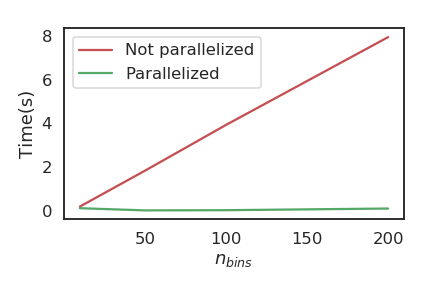
\includegraphics[width=0.5\textwidth]{normal_S.png}\label{fig:noarmalS}}
  \hfill
  \subfloat[Run time with $n$(sample size) as a variable.]{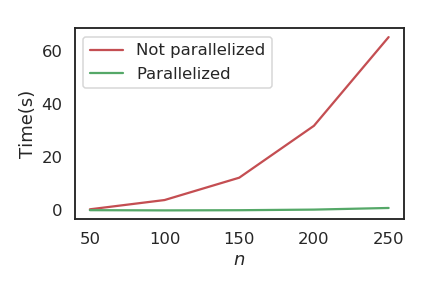
\includegraphics[width=0.5\textwidth]{normal_N.png}\label{fig:normalN}}
  \caption{Run time experiments.}
\end{figure}
\FloatBarrier
In the first experiment, $n_{bin}$ is the variable. Since $n_{bin}$ only changes range which $s$ can take on values, i.e., $0 \leq s \leq \mathcal{S}$, and from section \ref{sec:calcBottleneck} it's described that the run time is governed by $\mathcal{O}(m\cdot (m+n)\cdot \mathcal{S})$, and with everything fixed except $n_{bin}$, the algorithm scale linearly with $\mathcal{O}(\mathcal{S})$, which is demonstrated in the figure \ref{fig:noarmalS}.
In the second run time experiment, $n,m$ are the variables. Here $m=n$, therefore, the run time is $\mathcal{O}(n \cdot 2n)=\mathcal{O}(n^{2})$. This is demonstrated experimentally, see figure \ref{fig:normalN}.
In both cases, the parallelized version has almost constant run time, and this is because the GPU calculates everything at the same speed until it reaches its max capacity. If that would be the case, one has to re-load the GPU, which would require additional time. Hence, for more massive datasets, the GPU plot would look more like a step-function. 
\subsection{Calibration test}
The distributions used are $A \sim \mathcal{N}(0,1)$ and $B \sim \mathcal{N}(\mu,1)$ where $\boldsymbol{\mu} = \{0, 0.2, 0.4, \ldots, 1.8, 2.0 \}$(i.e., performing $11$ experiments.). For all $\mu \in \boldsymbol{\mu}$, 21 different bin sizes are tested $n_{bin}=\{10,12,14,\ldots,38,40\}$. For each bin size, the difference and relative error of the $p$-value between $t$-test and exact test (i.e., $p_{exact}-p_{t-test}$  and $\frac{p_{exact}-p_{t-test}}{p_{t-test}}$) are plotted against $n_{bin}$. Furthermore, these following hyperparameters for each experiment: the set size for both $A$ and $B$ is $100$ (i.e., $|A|=|B|=100$.), and the sample size is $70$.
\begin{figure}[H]
  \centering
  \subfloat[Boxplot of the relative error with bin size as varaible.]{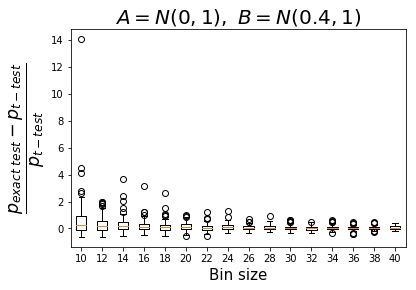
\includegraphics[width=0.5\textwidth]{box_plot_Diff_rel_2.jpg}\label{fig:noarmalS}}
  \hfill
  \subfloat[Errorplot of the relative error with bin size as varaible.]{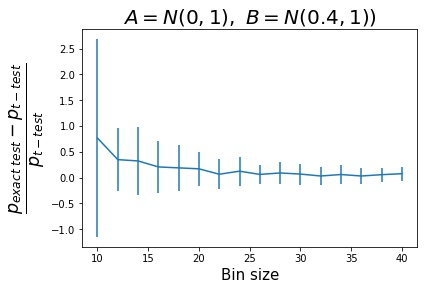
\includegraphics[width=0.5\textwidth]{error_plot_Diff_rel_2.jpg}\label{fig:normalN}}
  \caption{Relative error vs Bin size}
\end{figure}
\begin{figure}[H]
  \centering
  \subfloat[Boxplot of the relative error with bin size as varaible.]{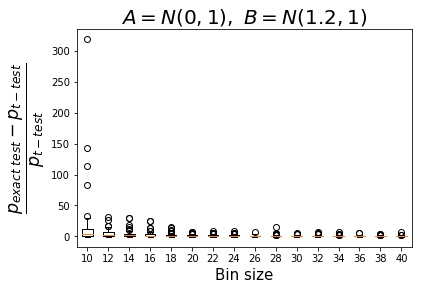
\includegraphics[width=0.5\textwidth]{box_plot_Diff_rel_6.jpg}\label{fig:noarmalS}}
  \hfill
  \subfloat[Errorplot of the relative error with bin size as varaible.]{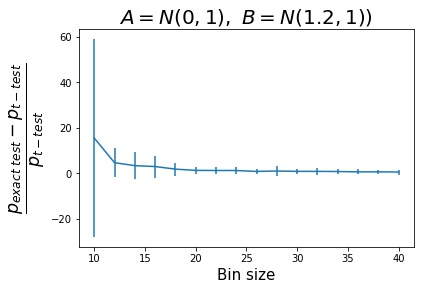
\includegraphics[width=0.5\textwidth]{error_plot_Diff_rel_6.jpg}\label{fig:normalN}}
  \caption{Relative error vs Bin size}
\end{figure}
{\bibliography{sample.bib}}
\bibliographystyle{ieeetr}
\end{document}